\section{Onvolmaakte Mededinging en Productdifferentiatie}

\subsection{Homogeen Oligopolie}
Een \textbf{oligopolie} is een marktvorm waarbij er wederzijdse be\"invloeding is $\Rightarrow$ gedrag mede bepaald door gedrag v/d concurrentie. Een \textbf{homogeen oligopolie} is een oligopolie waarin het product homogeen is.

We beginnen met het bespreken van een \textbf{homogeen duopolie}, waarbij beide ondernemingen dezelfde kostenstructuur hebben. Op het eerste zicht lijkt het een goed idee voor beiden om samen te werken en een kartel te vormen waarbij ze een $q^*$ bepalen die er voor zorgt dat hun winst zo hoog mogelijk is.
\todo[inline]{TODO: berekening slide 4 invoeren}
%\begin{align*}
%
%\end{align*}

We komen een evenwicht uit, maar beide spelers zullen een incentief hebben om hier van af te wijken. We maken eerst de berekening als A vals speelt en B zich aan de afspraak zal houden, maar ze zullen beiden meteen afwijken van de afspraak. Deze situatie berekenen we ook.
\todo[inline]{TODO: berekeningen slide 6 en 8 invoeren}
%\begin{align*}
%
%\end{align*}

Het uiteindelijke evenwicht dat zal onstaan, indien beide spelers \textbf{simultaan beslissen}, is het \textbf{Cournot-evenwicht}. Om dit evenwicht te bekomen zullen we de \textbf{reactiefunctie} voor beide spelers opstellen. Deze lossen we dan op in een stelsel en we bekomen het evenwicht.

Meestal zullen ondernemingen niet simultaan beslissen, maar zijn er een leider en een of meerdere volgers op de markt, waarbij de leider als eerste zijn hoeveelheid zal gaan zetten. De leider kent wel de reactiefuncties van de volgers en zal hier dus op anticiperen. Op basis van deze reactiefunctie(s) kan de leider dan een functie opstellen waarin enkel zijn eigen productie variabel is. Hij kan deze functie dan gaan maximaliseren. Het evenwicht dat hieruit ontstaat noemt men het \textbf{Stackelberg-evenwicht}.


\subsection{Oligopolie en Speltheorie}
De wederzijdse be\"invloeding in een oligopolie maakt dat we de markt ook kunnen analyseren aan de hand van spelteorie. Indien zoals voorheen geconcurreerd wordt via productievolumes, worden deze de mogelijke strategie\"en, er zijn er dan oneindig veel, en we zullen een Nash-evenwicht vinden in het punt waar we voorheen ook al het Cournot-evenwicht vonden.

Er kan ook geconcurreerd worden a.d.h.v. de prijs. In dit geval speelt de \textbf{paradox van Bertrand}. Indien alle ondernemingen dezelfde kostenstructuur hebben, zal de prijs dalen tot niemand nog winst maakt. Er wordt dus een resultaat gelijkwaardig aan dat van perfecte mededinging gerealiseerd terwijl slechts een klein aantal ondernemingen aanbieden.

Indien de ondernemingen niet dezelfde kostenstructuur hebben, zal degene met de laagste kostenstructuur de anderen wegconcurreren en er blijft een monopolie over.

\subsection{Productdifferentiatie}
\subsubsection{Monopolistische Mededinging}
Dit is de vierde marktvorm die besproken wordt en is een combinatie van monopolie en vrije mededinging. Het is een markt waar \textbf{heterogene goederen}(productdifferentiatie), die hetzelfde nut vervullen, verhandeld worden en zorgt ervoor dat alle ondernemingen prijszetters zijn. Er zijn wel veel aanbieders en vragers, vrije toe- en uittreding en er speelt geen interdependentie tussen de verschillende ondernemingen.

De vraagcurve is elastischer(vlakker) dan bij monopolie, maar niet perfect elastisch zoals bij vrije mededinging. Prijsveranderingen hebben dus meer effect dan bij monopolie, aangezien er nu goede substituten zijn. De prijszetting verloopt analoog aan het geval bij monopolie, zoals je kan zien in figuur~\ref{fig:prijszettingMCopKT}.

\begin{figure}[htbp]
   \centering
   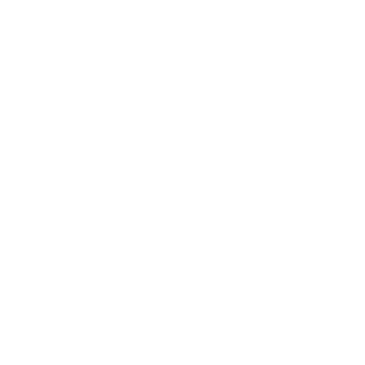
\includegraphics[scale=0.4]{Images/white.png}
   \caption{Prijszetting bij monopolistische concurrentie op KT (slide 22)}
   \label{fig:prijszettingMCopKT}
\end{figure}

Op lange termijn kunnen we er van uitgaan dat de vraagcurve vlakker wordt, zie figuur~\ref{fig:prijszettingMCopLT}, omdat zo lang winst gemaakt wordt, er nieuwe ondernemingen bij zullen komen. Met elke onderneming die er zo bij komt, neemt het aantal substituten toe voor alle andere ondernemingen en zal de vraag bij elke onderneming ook elastischer worden. Er zal dan een rusttoestand bereikt worden wanneer er geen winst meer gemaakt wordt.

\begin{figure}[htbp]
   \centering
   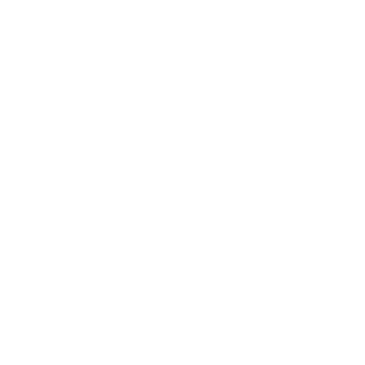
\includegraphics[scale=0.4]{Images/white.png}
   \caption{Prijszetting bij monopolistische concurrentie op LT (slide 24)}
   \label{fig:prijszettingMCopLT}
\end{figure}

\subsubsection{Heterogeen Oligopolie: Model van Hotelling}
Een heterogeen oligopolie is een markt van monopolistische concurrentie, met de wijziging dat er slechts een klein aantal aanbieders zijn. Er komt dus nog onderlinge afhankelijkheid voor de strategie van de ondernemingen bij. Om dit te analyseren gebruiken we het \textbf{model van Hotelling}.
\todo[inline]{TODO: meer schrijven over Hotelling}


\subsection{Asymmetrische Informatie}
We hadden het reeds over asymmetrische informatie in sectie~\ref{sssec:socialeInteracties} met het voorbeeld over de markt voor tweedehandswagens. Een ander voorbeeld is dat van verzekeringen. De verzekeringsnemer kent daar niet de gemiddelde risico's die de verzekeraar wel kent.
